 \documentclass[c]{beamer}
%\documentclass{beamer}
\listfiles

\mode<presentation>
{
  %\usetheme[deutsch,titlepage0]{KIT}
\usetheme[deutsch]{KIT}
% \usetheme{KIT}

%%  \usefonttheme{structurebold}

  \setbeamercovered{transparent}

  \setbeamertemplate{enumerate items}[circle]
  %\setbeamertemplate{enumerate items}[ball]

}
\usepackage{babel}
\date{}
%\DateText

\newlength{\Ku}
\setlength{\Ku}{1.43375pt}

\usepackage[utf8]{inputenc}
\usepackage[TS1,T1]{fontenc}
\usepackage{array}
\usepackage{multicol}
\usepackage{lipsum}
\usepackage[]{algorithm2e}
\usepackage{amsmath}
\usepackage{color}

\usenavigationsymbols
%\usenavigationsymbols[sfHhdb]
%\usenavigationsymbols[sfhHb]

\subtitle{Algorithmen I SS 14}
\author[]{Lena Winter}

\AuthorTitleSep{\relax}

\institute[ITI]{Institut für Theoretische Informatik}

\TitleImage[width=\titleimagewd]{images/title}

\newlength{\tmplen}

\newcommand{\verysmall}{\fontsize{6pt}{8.6pt}\selectfont}

\title[Algorithmen I SS 14]{Tutorium 4}

\usepackage{alltt}

\TitleImage[height=\titleimageht]{images/sortinghat}

\definecolor{english}{rgb}{0.0, 0.5, 0.0}

\begin{document}

\begin{frame}
  \maketitle
\end{frame}

\begin{frame} {Quicksort: Worst case}

	Letztes Tut: Worst case <=> Pivot ist immer Max/Min
	
	\begin{exampleblock} {Gedankenspiel:}
		Array bestehenend aus nur gleichen Elementen: \ \\
		\ \\
		\centerline{< 2, 2, 2, 2 >}
		\ \\
		Wie viele Vergleiche?
		\ \\
		\ \\
		$\rightarrow$ Auf Mengen mit vielen gleichen Elementen: \\
		\centerline{Standart-Quicksort schlecht}
		
	\end{exampleblock} 
\end{frame}

\begin{frame}{Stattdessen: 3-way-partition}
	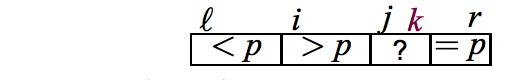
\includegraphics[width=10cm]{images/threeway} \\
	\begin{itemize}
		\item 3 Pointer: i, j ,k 
		\item Am Ende den ($ = p$) Teil zwischen ($< p$) und ($> p$) schieben.
	\end{itemize}

\end{frame}

\begin{frame}{Bucket sort}
	\begin{itemize}
		\item Array aus anfänglich leeren Buckets, denen jeweils ein Schlüssel zugewiesen ist
		\item Basierend auf den Schlüssel werden die Elemente in die Buckets sortiert
	\end{itemize}
	
	\begin{block}{Eigenschaften}
		{\color{english}{stabil}} \\
		{\color{red}{Nicht inplace}}: Im Worse case $\mathcal{O}(n * k)$ Komplexität\\
		Average Laufzeit $\mathcal{O}(n+k)$
	\end{block}
	
	
	$\rightarrow$ Sinnvoll bei kleiner Schlüsselmenge

\end{frame}

\begin{frame}{Radix sort}

	Sortieren nach einzelnen Ziffern \\
	Mehrere Varianten:
	\begin{itemize}
		\item Beginnend beim Most Significant Digit
		\item Beginnend beim Least Significant Digit
	\end{itemize}
	
	\begin{block}{Eigenschaften}
		{\color{english}{stabil}}\\
		{\color{red}{Nicht inplace}}: Worse case $\Theta(d * (n + k))$ Komplexität\\
		Laufzeit $\mathcal{O}(d * n)$ für d $=$ Anzahl digits
	\end{block}
	
	
	$\rightarrow$ Sinnvoll bei kleiner Wertmenge

\end{frame}

\begin{frame}{Vergleichsbasiert vs. Nicht Vergleichsbasiert}
	
	{\textbf{\large{Pro Nicht Vergleichsbasiert:}}}
	\begin{itemize}
		\item asymptotisch schneller
	\end{itemize}

	
	{\textbf{\large{Pro Vergleichsbasiert:}}} \\
	\begin{itemize}
		\item Weniger Voraussetzungen an die zu sortierenden Elemente
		\item Cache-Effizienz weniger schwierig
		\item bei langen Schlüsseln oft schneller
		\item robust gegen beliebige Eingabeverteilungen
	\end{itemize}

\end{frame}


\end{document}
